\documentclass[11pt]{article}

\usepackage[letterpaper,margin=0.75in]{geometry}
\usepackage{booktabs}
\usepackage{caption}
\usepackage{graphicx}
\usepackage{listings}
\usepackage{float}
\usepackage{scrextend}
\usepackage{hyperref}
\usepackage[parfill]{parskip}
\renewcommand{\lstlistingname}{Snippet}


\begin{document}

\lstset{
  language=Python,
  basicstyle=\small,          % print whole listing small
  keywordstyle=\bfseries,
  identifierstyle=,           % nothing happens
  commentstyle=,              % white comments
  stringstyle=\ttfamily,      % typewriter type for strings
  showstringspaces=false,     % no special string spaces
  numbers=left,
  numberstyle=\tiny,
  numbersep=5pt,
  frame=tb,
}

\title{Congestion Control Part 1}

\author{Brandt Elison & Joe Eklund}

\date{March 16, 2016}

\maketitle

\section{Test Results}


\begin{enumerate}
  \item Slow Start
  
\begin{figure}[H]
\caption{The graph of our slow start output test.}
	\label{figure1}
  	\centering
  	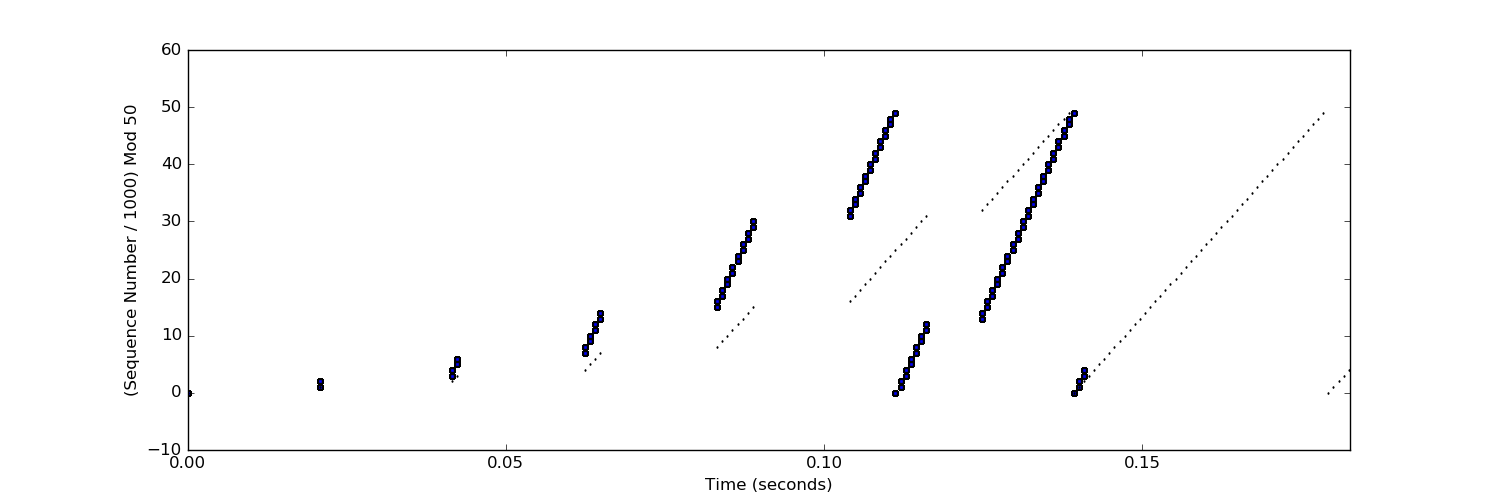
\includegraphics{figure1}
\end{figure}

%discuss slow start here

  \item Additive Increase
  
  \begin{figure}[H]
\caption{The graph of our additive increase output test.}
	\label{figure2}
  	\centering
  	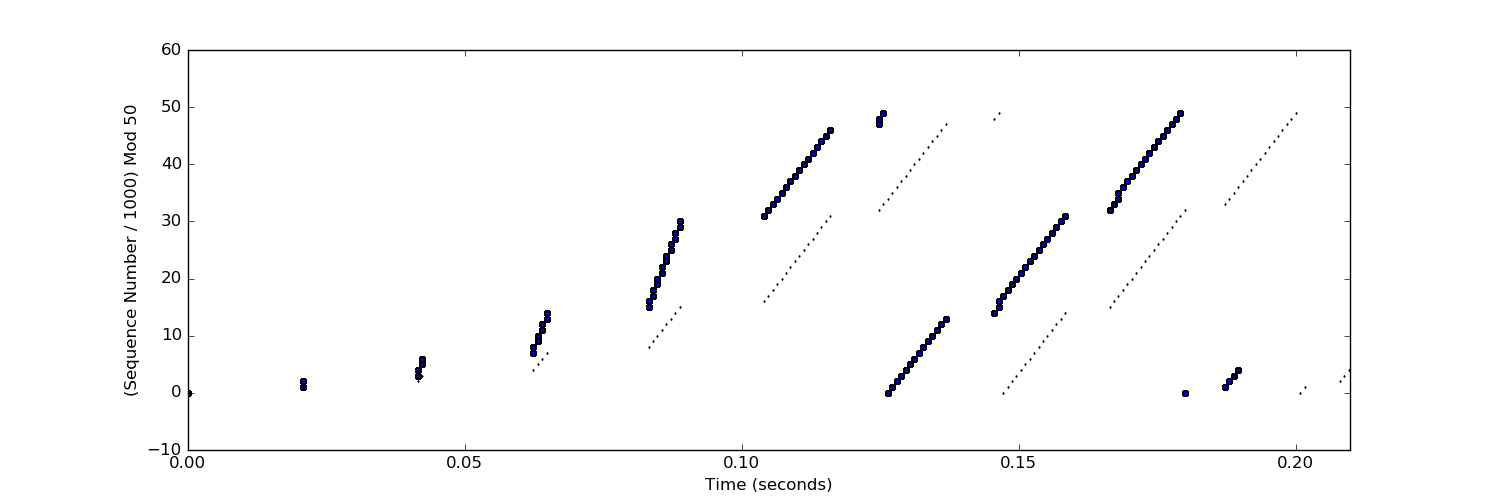
\includegraphics{figure2}
\end{figure}

%discuss additive increase here

  \item AIMD

\begin{figure}[H]
\caption{The graph of our AIMD output test.}
	\label{figure3}
  	\centering
  	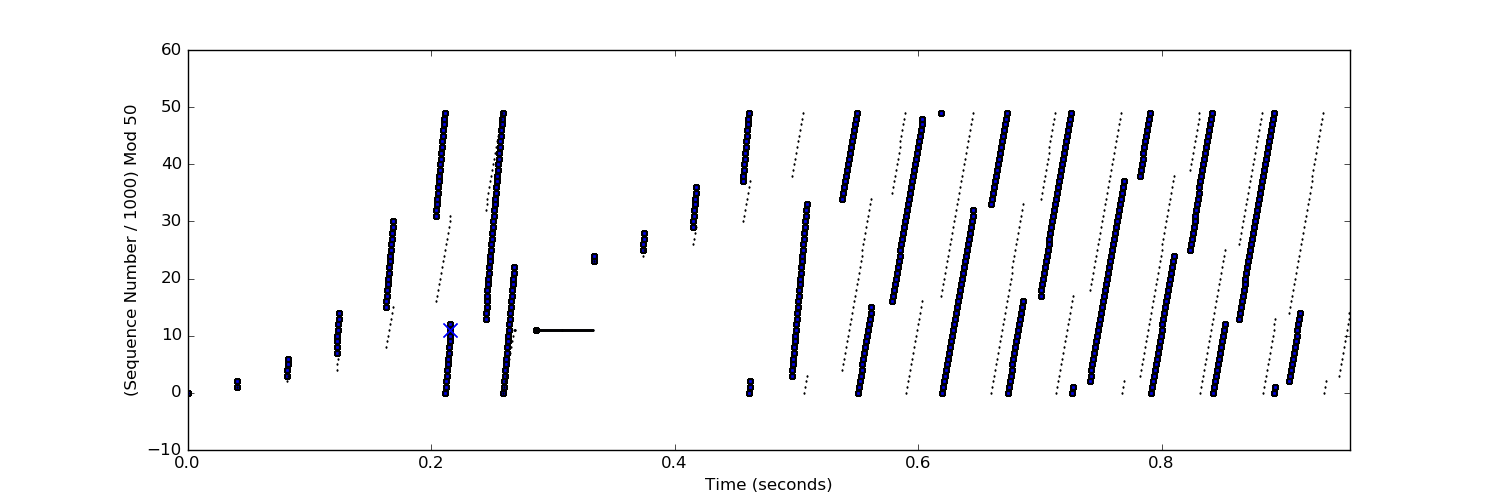
\includegraphics{figure3}
\end{figure}

%discuss AIMD here

  \item Burst Loss

\begin{figure}[H]
\caption{The graph of our burst loss output test.}
	\label{figure4}
  	\centering
  	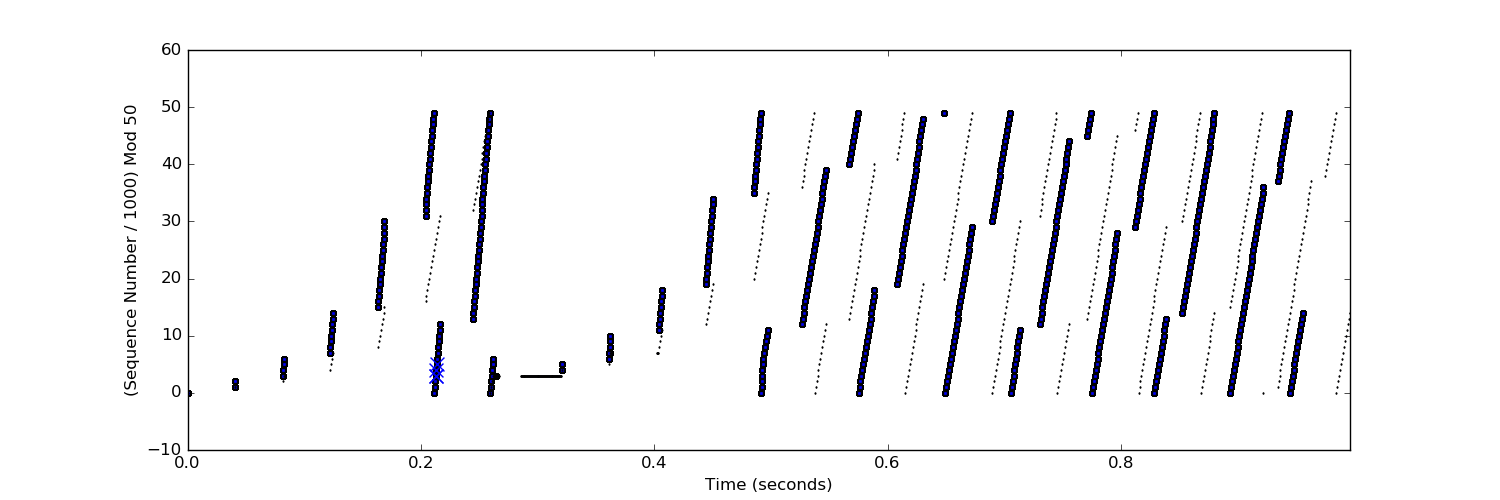
\includegraphics{figure4}
\end{figure}

%discuss burst loss

\end{enumerate}


\end{document}
